
\documentclass{article}

\usepackage{graphicx}
\graphicspath{ {../res/} }





%%%%%%%%%%%%%%%%%%%%%%%%%%%%%%%%%%%%%%%%%
% Lachaise Assignment
% Structure Specification File
% Version 1.0 (26/6/2018)
%
% This template originates from:
% http://www.LaTeXTemplates.com
%
% Authors:
% Marion Lachaise & François Févotte
% Vel (vel@LaTeXTemplates.com)
%
% License:
% CC BY-NC-SA 3.0 (http://creativecommons.org/licenses/by-nc-sa/3.0/)
% 
%%%%%%%%%%%%%%%%%%%%%%%%%%%%%%%%%%%%%%%%%

%----------------------------------------------------------------------------------------
%	PACKAGES AND OTHER DOCUMENT CONFIGURATIONS
%----------------------------------------------------------------------------------------

\usepackage{amsmath,amsfonts,stmaryrd,amssymb} % Math packages

\usepackage{enumerate} % Custom item numbers for enumerations

\usepackage[ruled]{algorithm2e} % Algorithms

\usepackage[framemethod=tikz]{mdframed} % Allows defining custom boxed/framed environments

\usepackage{listings} % File listings, with syntax highlighting
\lstset{
	basicstyle=\ttfamily, % Typeset listings in monospace font
}

%----------------------------------------------------------------------------------------
%	DOCUMENT MARGINS
%----------------------------------------------------------------------------------------

\usepackage{geometry} % Required for adjusting page dimensions and margins

\geometry{
	paper=a4paper, % Paper size, change to letterpaper for US letter size
	top=2.5cm, % Top margin
	bottom=3cm, % Bottom margin
	left=2.5cm, % Left margin
	right=2.5cm, % Right margin
	headheight=14pt, % Header height
	footskip=1.5cm, % Space from the bottom margin to the baseline of the footer
	headsep=1.2cm, % Space from the top margin to the baseline of the header
	%showframe, % Uncomment to show how the type block is set on the page
}

%----------------------------------------------------------------------------------------
%	FONTS
%----------------------------------------------------------------------------------------

\usepackage[utf8]{inputenc} % Required for inputting international characters
\usepackage[T1]{fontenc} % Output font encoding for international characters

\usepackage{XCharter} % Use the XCharter fonts

%----------------------------------------------------------------------------------------
%	COMMAND LINE ENVIRONMENT
%----------------------------------------------------------------------------------------

% Usage:
% \begin{commandline}
%	\begin{verbatim}
%		$ ls
%		
%		Applications	Desktop	...
%	\end{verbatim}
% \end{commandline}

\mdfdefinestyle{commandline}{
	leftmargin=10pt,
	rightmargin=10pt,
	innerleftmargin=15pt,
	middlelinecolor=black!50!white,
	middlelinewidth=2pt,
	frametitlerule=false,
	backgroundcolor=black!5!white,
	frametitle={Command Line},
	frametitlefont={\normalfont\sffamily\color{white}\hspace{-1em}},
	frametitlebackgroundcolor=black!50!white,
	nobreak,
}

% Define a custom environment for command-line snapshots
\newenvironment{commandline}{
	\medskip
	\begin{mdframed}[style=commandline]
}{
	\end{mdframed}
	\medskip
}

%----------------------------------------------------------------------------------------
%	FILE CONTENTS ENVIRONMENT
%----------------------------------------------------------------------------------------

% Usage:
% \begin{file}[optional filename, defaults to "File"]
%	File contents, for example, with a listings environment
% \end{file}

\mdfdefinestyle{file}{
	innertopmargin=1.6\baselineskip,
	innerbottommargin=0.8\baselineskip,
	topline=false, bottomline=false,
	leftline=false, rightline=false,
	leftmargin=2cm,
	rightmargin=2cm,
	singleextra={%
		\draw[fill=black!10!white](P)++(0,-1.2em)rectangle(P-|O);
		\node[anchor=north west]
		at(P-|O){\ttfamily\mdfilename};
		%
		\def\l{3em}
		\draw(O-|P)++(-\l,0)--++(\l,\l)--(P)--(P-|O)--(O)--cycle;
		\draw(O-|P)++(-\l,0)--++(0,\l)--++(\l,0);
	},
	nobreak,
}

% Define a custom environment for file contents
\newenvironment{file}[1][File]{ % Set the default filename to "File"
	\medskip
	\newcommand{\mdfilename}{#1}
	\begin{mdframed}[style=file]
}{
	\end{mdframed}
	\medskip
}

%----------------------------------------------------------------------------------------
%	NUMBERED QUESTIONS ENVIRONMENT
%----------------------------------------------------------------------------------------

% Usage:
% \begin{question}[optional title]
%	Question contents
% \end{question}

\mdfdefinestyle{question}{
	innertopmargin=1.2\baselineskip,
	innerbottommargin=0.8\baselineskip,
	roundcorner=5pt,
	nobreak,
	singleextra={%
		\draw(P-|O)node[xshift=1em,anchor=west,fill=white,draw,rounded corners=5pt]{%
		Question \theQuestion\questionTitle};
	},
}

\newcounter{Question} % Stores the current question number that gets iterated with each new question

% Define a custom environment for numbered questions
\newenvironment{question}[1][\unskip]{
	\bigskip
	\stepcounter{Question}
	\newcommand{\questionTitle}{~#1}
	\begin{mdframed}[style=question]
}{
	\end{mdframed}
	\medskip
}

%----------------------------------------------------------------------------------------
%	WARNING TEXT ENVIRONMENT
%----------------------------------------------------------------------------------------

% Usage:
% \begin{warn}[optional title, defaults to "Warning:"]
%	Contents
% \end{warn}

\mdfdefinestyle{warning}{
	topline=false, bottomline=false,
	leftline=false, rightline=false,
	nobreak,
	singleextra={%
		\draw(P-|O)++(-0.5em,0)node(tmp1){};
		\draw(P-|O)++(0.5em,0)node(tmp2){};
		\fill[black,rotate around={45:(P-|O)}](tmp1)rectangle(tmp2);
		\node at(P-|O){\color{white}\scriptsize\bf !};
		\draw[very thick](P-|O)++(0,-1em)--(O);%--(O-|P);
	}
}

% Define a custom environment for warning text
\newenvironment{warn}[1][Warning:]{ % Set the default warning to "Warning:"
	\medskip
	\begin{mdframed}[style=warning]
		\noindent{\textbf{#1}}
}{
	\end{mdframed}
}

%----------------------------------------------------------------------------------------
%	INFORMATION ENVIRONMENT
%----------------------------------------------------------------------------------------

% Usage:
% \begin{info}[optional title, defaults to "Info:"]
% 	contents
% 	\end{info}

\mdfdefinestyle{info}{%
	topline=false, bottomline=false,
	leftline=false, rightline=false,
	nobreak,
	singleextra={%
		\fill[black](P-|O)circle[radius=0.4em];
		\node at(P-|O){\color{white}\scriptsize\bf i};
		\draw[very thick](P-|O)++(0,-0.8em)--(O);%--(O-|P);
	}
}

% Define a custom environment for information
\newenvironment{info}[1][Info:]{ % Set the default title to "Info:"
	\medskip
	\begin{mdframed}[style=info]
		\noindent{\textbf{#1}}
}{
	\end{mdframed}
}
 % Include the file specifying the document structure and custom commands

%----------------------------------------------------------------------------------------
%	ASSIGNMENT INFORMATION
%----------------------------------------------------------------------------------------

\title{Práctica 1: Filtrado y Muestreo} % Title of the assignment

\author{David Gil Bautista\\ \texttt{DNI: 45925424M}} % Author name and email address

\date{Universidad de Granada --- \today} % University, school and/or department name(s) and a date

%----------------------------------------------------------------------------------------

\begin{document}

\maketitle % Print the title

%----------------------------------------------------------------------------------------
%	INTRODUCTION
%----------------------------------------------------------------------------------------

\section{Funciones OpenCV} % Unnumbered section

USANDO LAS FUNCIONES DE OPENCV : escribir funciones que implementen los siguientes puntos:

\subsection{El cálculo de la convolución de una imagen con una máscara Gaussiana 2D (Usar GaussianBlur). Mostrar ejemplos con distintos tamaños de máscara y valores de sigma. Valorar los resultados.}

Para resolver este apartado debemos saber cómo funciona una máscara Gaussiana, y para ello mostraré el siguiente gráfico que nos ayudará a comprender mejor el concepto.

\begin{figure}[h]

\centering
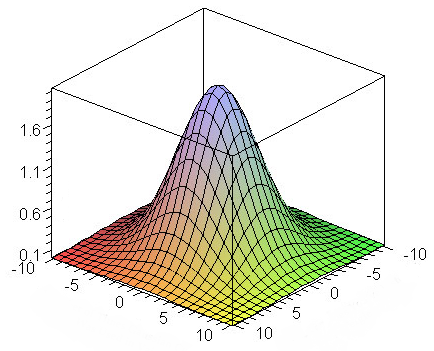
\includegraphics{gauss.PNG}
\caption{Campana de Gauss en 3D}
\label{fig:gauss}

\end{figure}

Una máscara Gaussiana presenta un kernel que es una aproximación en dos dimensiones de una función Gaussiana.

\begin{equation}
h(u,v) = \frac{1}{2\pi\sigma^2}e^{-\frac{u^2+v^2}{\sigma^2}}
\end{equation}

En nuestro caso el kernel nos permitirá escoger el tamaño de la máscara con el que trabajaremos, y para ello probaremos con los siguientes tamaños 1, 3, 5 y 7 píxeles.  Un tamaño de 5 píxeles quiere decir que trabajaremos con el pixel central y dos a su izquierda y derecha, es decir, siendo x el pixel central y k el tamaño de la máscara, trabajaremos con las siguientes posiciones:

\begin{equation}
x\pm\frac{(k-1)}{2}+1
\end{equation}

La varianza, por definición es la desviación estandar al cuadrado. Esta desviación nos indica lo dispersos que están los elementos respecto de la media. Una función con una varianza alta hace que la función sea más plana y que los datos no estén tan cerca de la media. Sabiendo esto podemos decir que cuanto menor sea la varianza vamos a tener más ceros en el mismo kernel, por lo que estos datos serán menos relevantes.


\begin{figure}[h]

\centering
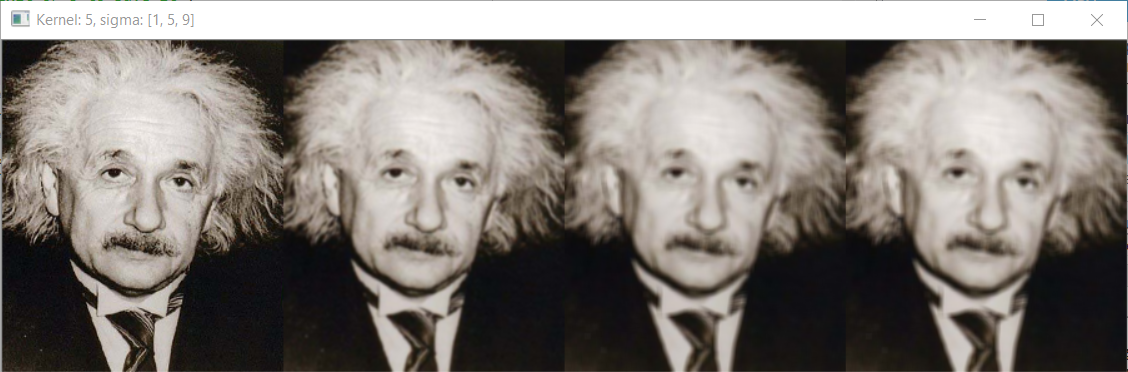
\includegraphics[scale=0.58]{1a1.PNG}
\caption{Kernel = 5, Sigma = 1,5,9}

\end{figure}

\begin{figure}[h]

\centering
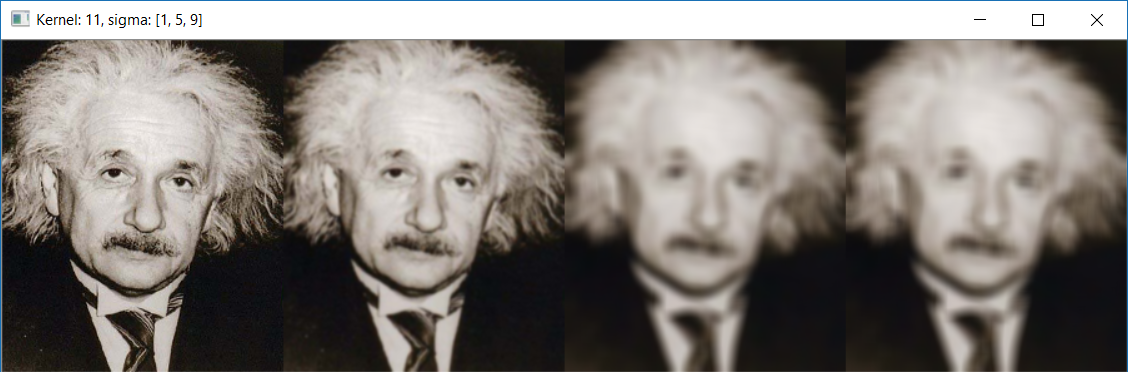
\includegraphics[scale=0.58]{1a2.PNG}
\caption{Kernel = 9, Sigma = 1,5,9}
\end{figure}

\begin{figure}[h]

\centering
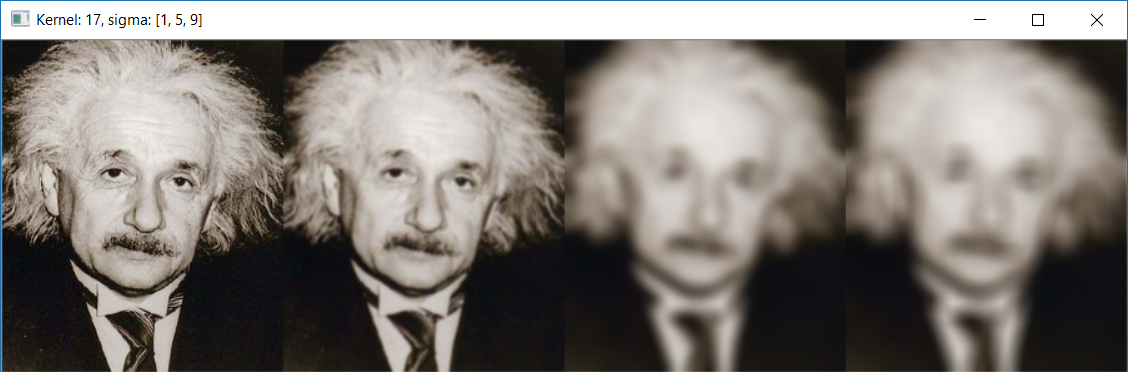
\includegraphics[scale=0.58]{1a3.PNG}
\caption{Kernel = 17, Sigma = 1,5,9}
\end{figure}

Como podemos ver en las imágenes mostradas, conforme aumentamos el tamaño del kernel y la varianza vamos obteniendo un desenfoque mayor.



\newpage
\subsection{ Usar getDerivKernels para obtener las máscaras 1D que permiten calcular al convolución 2D con máscaras de derivadas. Representar e interpretar dichas máscaras 1D para distintos valores de sigma.}

Para este apartado se usa la función getDerivKernels para obtener las máscaras de derivadas que podemos usar para calcular la convolución en 2D. Para ello he probado con distintos tamaños de máscara y he escogido la máscara de la derivada respecto a y para calcular la convolución en dos dimensiones y aplicar un filtro de alisamiento.

\begin{figure}[h]

\centering
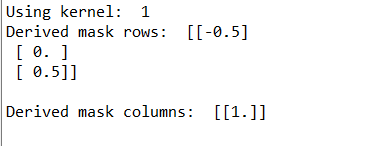
\includegraphics[scale=1.1]{1b1.PNG}
\caption{Tamaño de kernel = 1}
\end{figure}

Para un kernel de tamaño 1 obtenemos una convolución con un único dato de valor 1, y al aplicar el filtro a una imagen obtenemos otra imagen exactamente igual puesto que al evaluar los píxeles estos toman su mismo valor.

Aquí podemos ver la representación gráfica.

\begin{figure}[h]
\centering
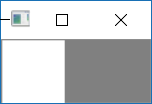
\includegraphics[scale=1.1]{1b11.PNG}
\caption{Convolución k=1}
\end{figure}

A medida que vamos cambiando el tamaño del kernel obtenemos una matriz en la que los valores se van atenuando más conforme se separan de la media.

En las siguientes imágenes podemos ver las máscaras 1D para un tamaño de kernel de 5 píxeles y las distintas representaciones de la convolución para otros tamaños adicionales.

\begin{figure}[h]
\centering
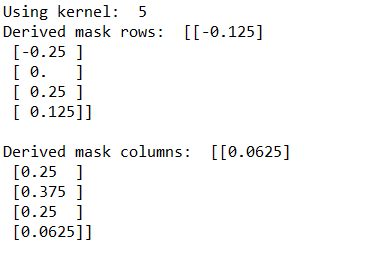
\includegraphics[scale=1]{1b3.PNG}
\caption{Máscaras derivadas 1D con k=5}
\end{figure}

Para la representación de las siguientes convoluciones para tamaños de kernel de 3, 5 y 7 se ha multiplicado el resultado final por un número positivo para que el filtro se aprecie mejor.

\begin{figure}[h]
\begin{minipage}[b]{0.2\linewidth}
\centering
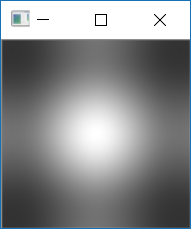
\includegraphics[scale=0.5]{1b22.PNG}
\caption{Kernel = 3}	
\end{minipage}
\begin{minipage}[b]{0.5\linewidth}
\centering
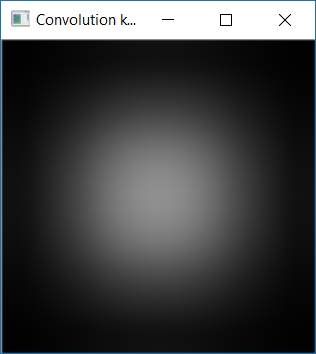
\includegraphics[scale=0.45]{1b33.PNG}
\caption{Kernel = 5}
\end{minipage}
\hspace{0.6cm}
\begin{minipage}[b]{0.1\linewidth}
\centering
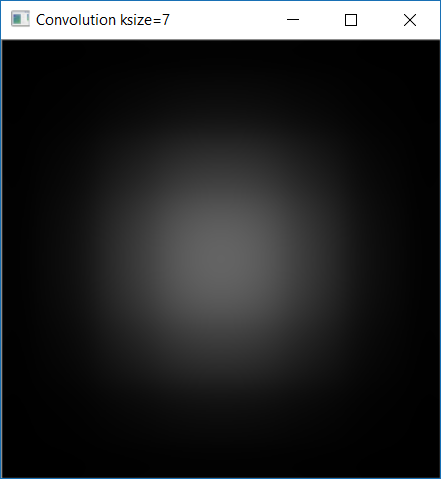
\includegraphics[scale=0.45]{1b44.PNG}
\caption{Kernel = 7}
\end{minipage}
\end{figure}


Conforme aumentamos el tamaño del kernel podemos ver que el área de desenfoque se distribuye más y que los píxeles centrales a la media son menos relevantes que con un tamaño de máscara menor. De esta forma podemos ver gráficamente lo que hemos realizado en el apartado anterior donde para una misma varianza el tamaño de la máscara es proporcional al desenfoque que obtenemos.	

\newpage
\subsection{Usar la función Laplacian para el cálculo de la convolución 2D con una máscara de Laplaciana-de-Gaussiana de tamaño variable. Mostrar ejemplos de funcionamiento usando dos tipos de bordes y dos valores de sigma: 1 y 3}

Para este ejercicio hemos usado la función Laplaciana para detectar los bordes de una imagen y también la derivada parcial de la imagen para ver qué método es más efectivo.


\begin{figure}[h]
\centering
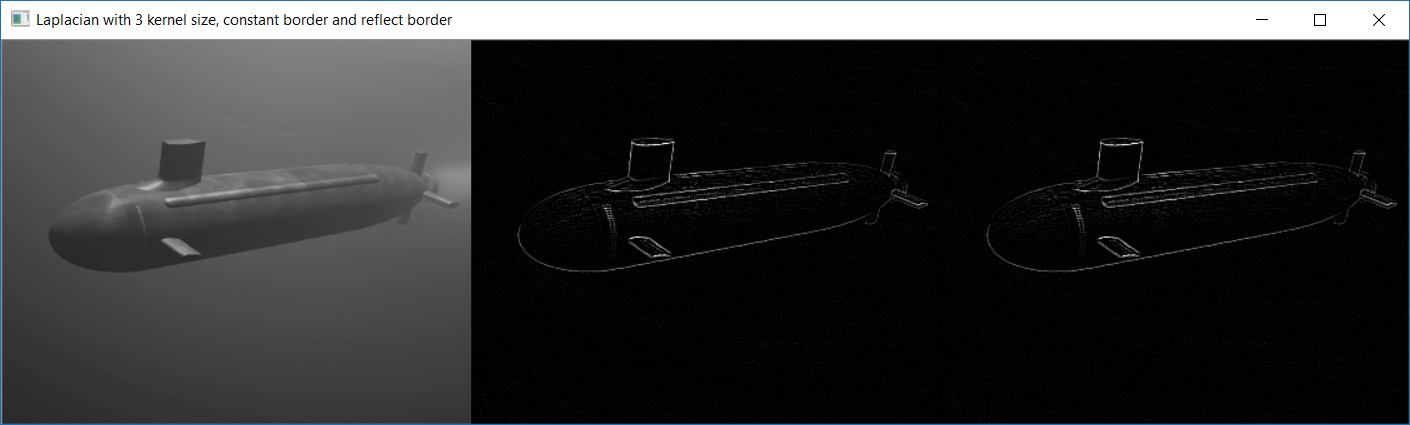
\includegraphics[scale=0.5]{1c1.PNG}
\caption{Función laplaciana con kernel = 3}
\end{figure}


\begin{figure}[h]
\centering
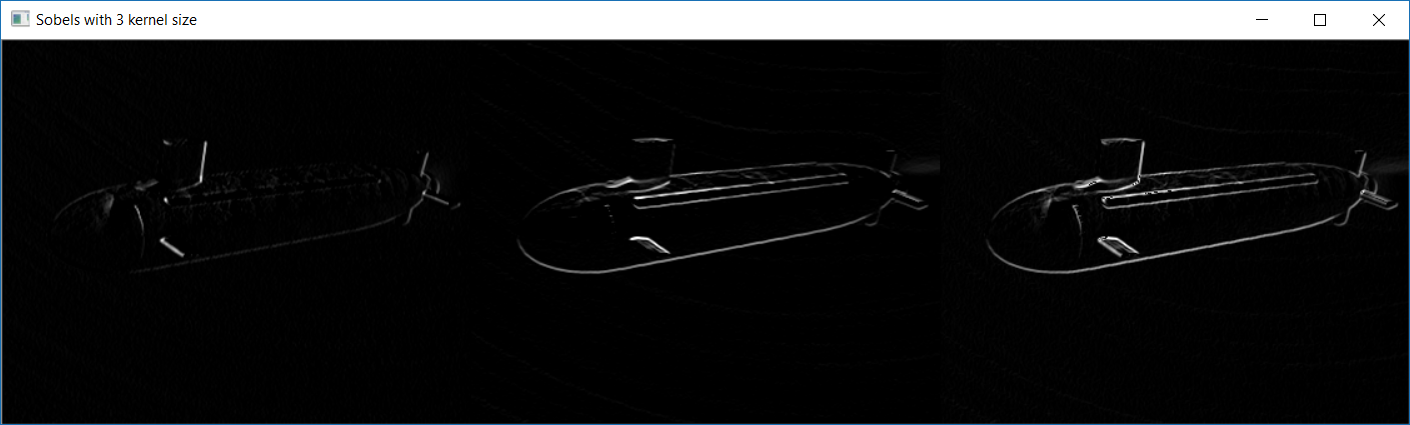
\includegraphics[scale=0.5]{1c2.PNG}
\caption{Función sobels con kernel = 3}
\end{figure}

Para un tamaño de máscara de 3 píxeles podemos ver que la función Laplaciana con dos tipos distintos de bordes nos ofrece un resultado similar. El escoger un determinado tipo de bordes nos ayuda a conseguir un resultado más fiable en una imagen en la cual nos encontramos con detalles en los bordes y que podemos perder en caso de rellenar el borde con un color sólido, pero en este caso los resultados han sido idénticos.

Respecto a los bordes de los objetos encontrados, podemos apreciar que la función laplaciana nos da unos bordes más finos y con más detalle, mientras que la suma de las derivadas parciales reconoce bien los bordes pero nos da un resultado más tosco.

\begin{figure}[h]
\centering
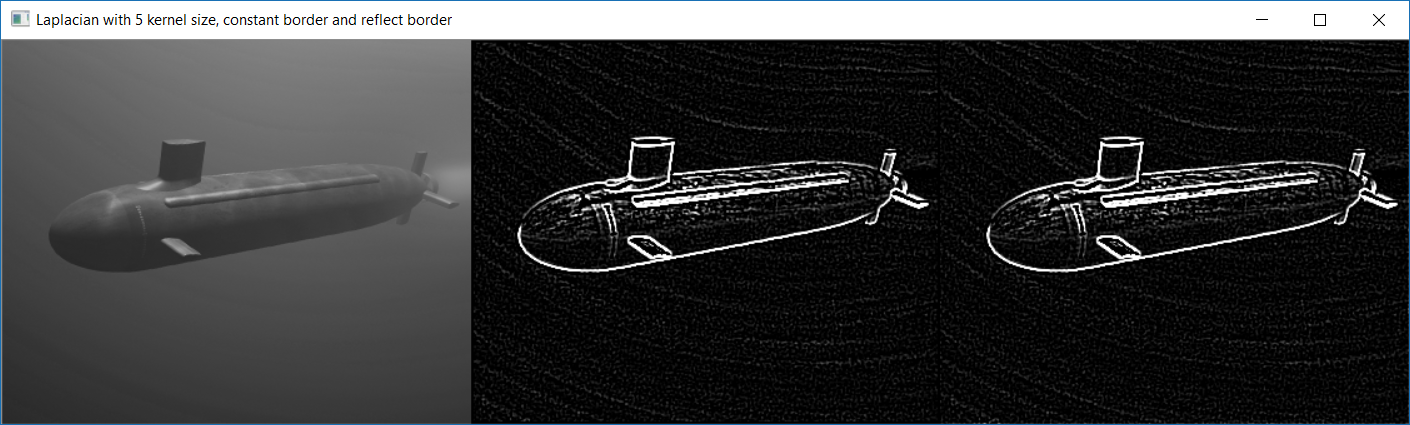
\includegraphics[scale=0.5]{1c3.PNG}
\caption{Función laplaciana con kernel = 5}
\end{figure}


\begin{figure}[h]
\centering
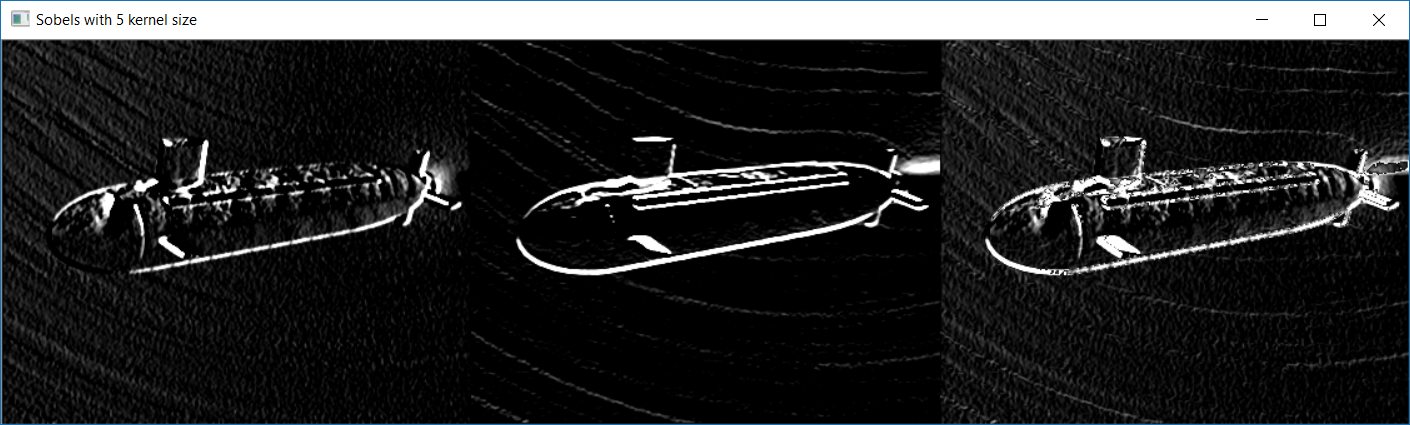
\includegraphics[scale=0.5]{1c4.PNG}
\caption{Función sobels con kernel = 5}
\end{figure}


Al aumentar el tamaño del kernel podemos ver que la función laplaciana ha hecho más gordos los bordes que ya había encontrado con un tamaño de kernel menor y que muestra ciertos detalles que antes no se apreciaban, a pesar de mostrar un poco más de ruido.

Usando las derivadas parciales generamos mucho ruido en el objeto, debido a las luces y sombras, y en la propia escena. Al sumar las derivadas obtenemos una imagen con mucho ruido y rugosidad. Por lo que podemos determinar que la función Laplaciana nos ofrece mejores resultados.



\newpage
\section{Convolución y pirámides} % Numbered section

Implementar apoyándose en las funciones \textit{getDerivKernels}, \textit{getGaussianKernel}, \textit{pyrUp}(), \textit{pyrDown}(), escribir funciones los siguientes:

%------------------------------------------------

\subsection{El cálculo de la convolución 2D con una máscara separable de tamaño variable. Usar bordes reflejados. Mostrar resultados.}

Para el desarrollo de este apartado he optado por usar \textit{getGaussianKernel} para obtener una máscara separable de tamaño \textbf{k} y \textbf{sigma} fijo en 3.

Una vez usamos la función y obtenemos nuestro kernel calculamos la convolución como la multiplicación de la máscara por su traspuesta y la aplicamos usando la función \textit{filter2D} con bordes constantes (bordes negros)

\begin{figure}[h]
\begin{minipage}[b]{0.5\linewidth}
\centering
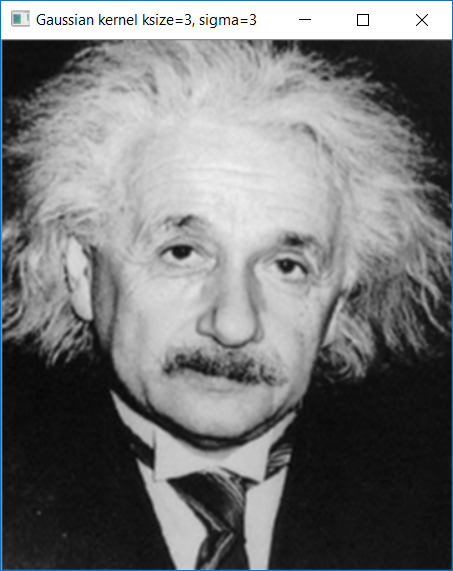
\includegraphics[scale=0.5]{2a1.PNG}
\caption{Kernel = 3}	
\end{minipage}
\begin{minipage}[b]{0.5\linewidth}
\centering
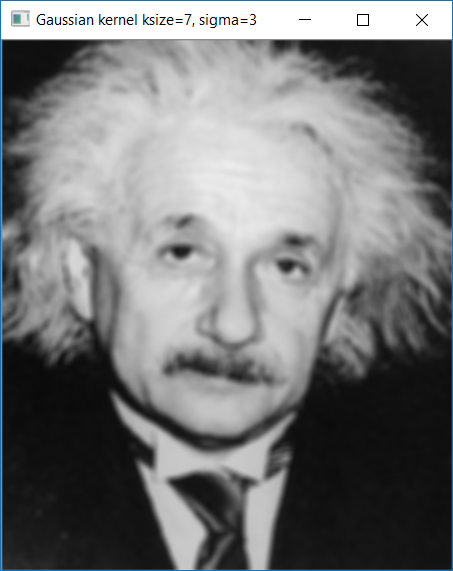
\includegraphics[scale=0.5]{2a2.PNG}
\caption{Kernel = 7}
\end{minipage}

\end{figure}

\begin{figure}[h]
\centering
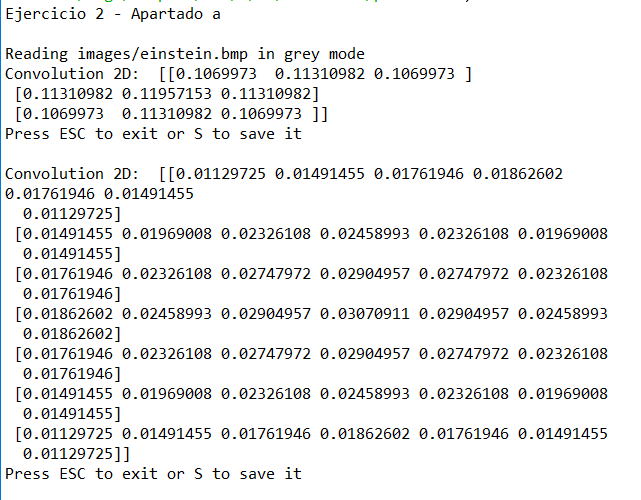
\includegraphics[scale=0.8]{2a3.PNG}
\caption{Convolución para k=3 y k=7}
\end{figure}


\newpage
Como se puede comprobar en esta última imagen obtenemos dos matrices gaussianas en las que podemos apreciar que en la primera, con un tamaño del kernel de 3 pixeles, apenas hay diferencia entre los valores de la matriz, pero en la segunda, con un tamaño de 7 pixeles, se nota más la diferencia con los puntos que están más alejados de la media.


\newpage
\subsection{El cálculo de la convolución 2D con una máscara 2D de 1ª derivada de tamaño variable. Mostrar ejemplos de funcionamiento usando bordes a cero.}

En este apartado usamos \textit{getDerivKernels} para obtener una máscara de primera derivada con un tamaño variable de k. El uso de la primera derivada nos permite calcular los saltos que hay en las fronteras y realzarlos.

\begin{figure}[h]
\centering
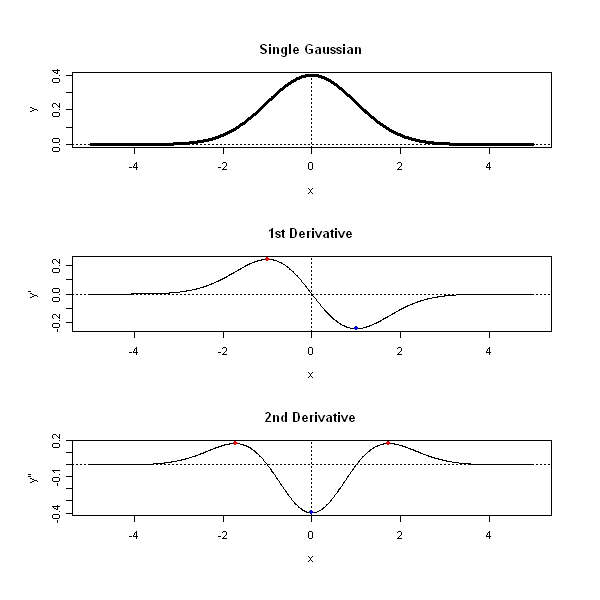
\includegraphics[scale=0.5]{2b3.PNG}
\caption{Derivadas}
\end{figure}

La primera derivada realza las partes de una imagen donde encontramos un contraste mayor, y esto suele darse en las fronteras donde la información los pixeles suele ser muy diferente.



\begin{figure}[h]
\centering
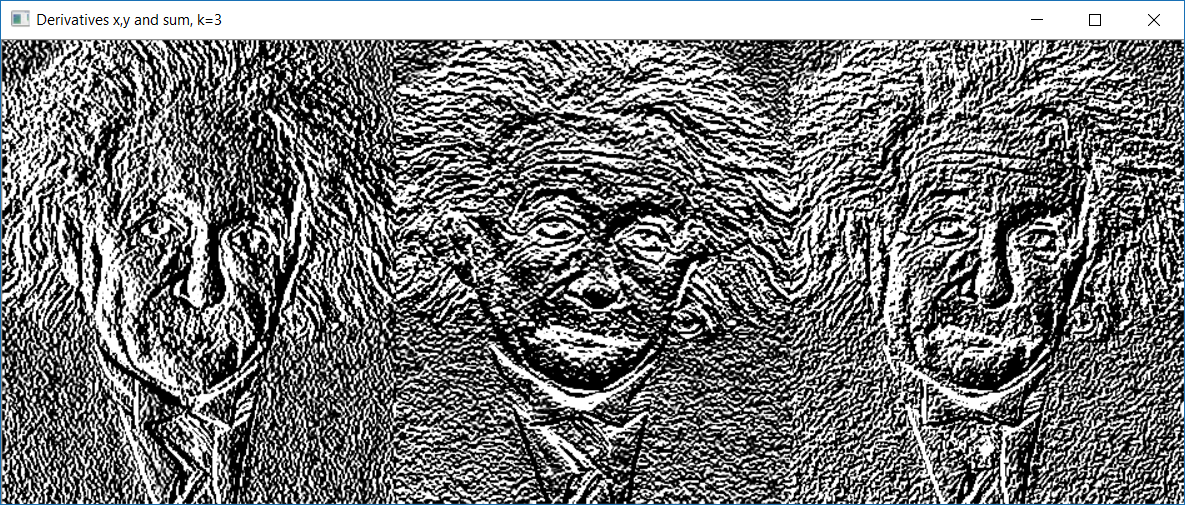
\includegraphics[scale=0.5]{2b1.PNG}
\caption{Primera derivada k=3}
\end{figure}


\begin{figure}[h]
\centering
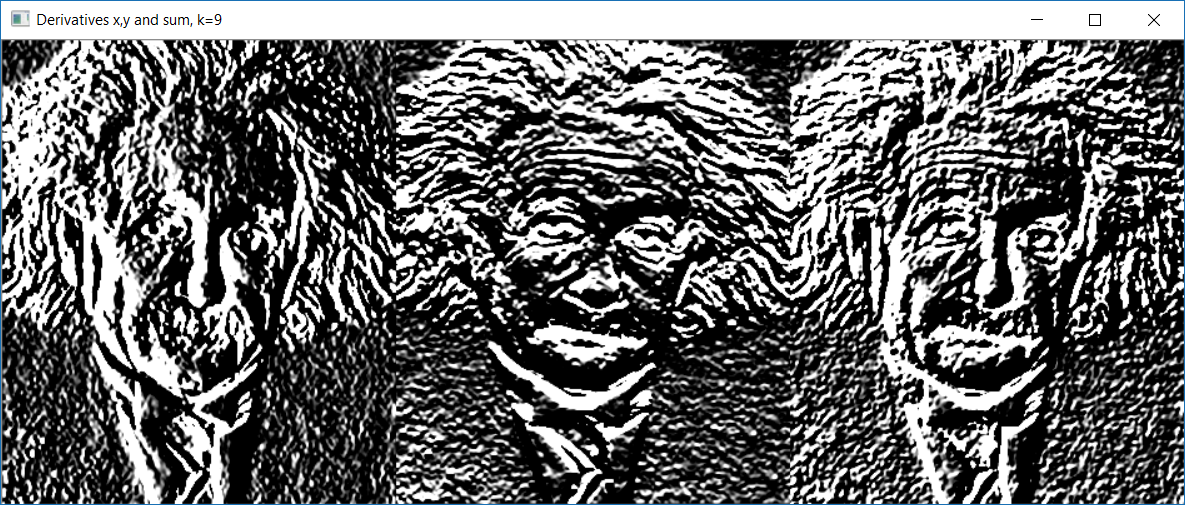
\includegraphics[scale=0.5]{2b2.PNG}
\caption{Primera derivada k=9}
\end{figure}



Conforme aumentamos el tamaño de la máscara usamos más valores para operar con la derivada y en este caso hacemos que los saltos sean más grandes.


\newpage
\subsection{El cálculo de la convolución 2D con una máscara 2D de 2ª derivada de tamaño variable. }

En este apartado volvemos a usar \textit{getDerivKernels} pero esta vez usando la segunda derivada para para crear una máscara con tamaño k.

En el apartado anterior hemos podido ver la forma que tiene la segunda derivada, dicha máscara realza un pixel central sobre los contiguos al mismo. De esta forma también conseguimos realzar las fronteras en una imagen.

\begin{figure}[h]
\begin{minipage}[b]{0.5\linewidth}
\centering
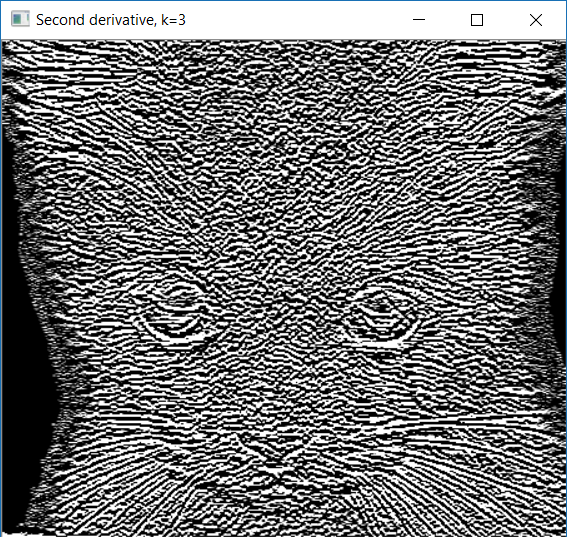
\includegraphics[scale=0.5]{2c1.PNG}
\caption{Kernel = 3}	
\end{minipage}
\begin{minipage}[b]{0.5\linewidth}
\centering
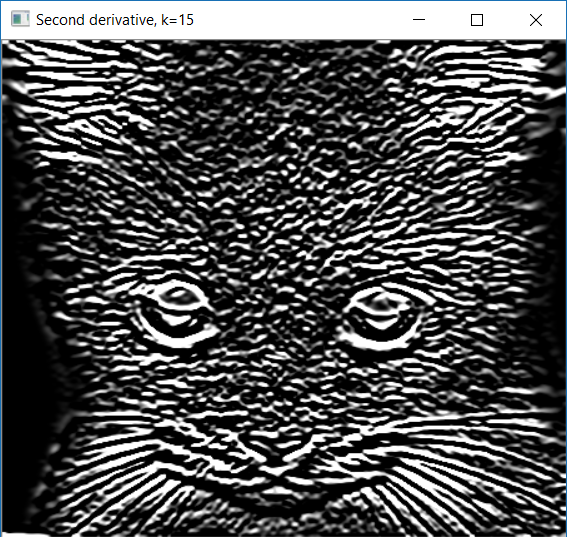
\includegraphics[scale=0.5]{2c2.PNG}
\caption{Kernel = 15}
\end{minipage}
\end{figure}


Al igual que en el caso anterior conforme aumentamos el tamaño del kernel los saltos entre las fronteras son más pronunciados por lo que a pesar de representar aquellas fronteras más relevantes perdemos detalle en las que son menos apreciables.

\newpage
\subsection{Una función que genere una representación en pirámide Gaussiana de 4 niveles de una imagen. Mostrar ejemplos de funcionamiento usando bordes.}
Con una pirámide Gaussiana representamos cómo se vería una imagen al hacerla más pequeña y después volver a escalarla al tamaño anterior. Haciendo esto podemos ver que en cada nivel la imagen tiene menos calidad debido que al hacer más pequeña la imagen estamos perdiendo información ya que no vamos a poder ver todos los píxeles que teníamos antes, y al volver a escalarla interpolamos menos información a un tamaño mayor, por lo que podemos ver gráficamente cómo va empeorando con el paso de los niveles.

Se ha realizado con dos tipos de bordes, el borde por defecto que tiene OpenCV y el borde reflejado que replica la información de las fronteras de la imagen. El resultado es similar para ambos bordes.


\begin{figure}[h]
\centering
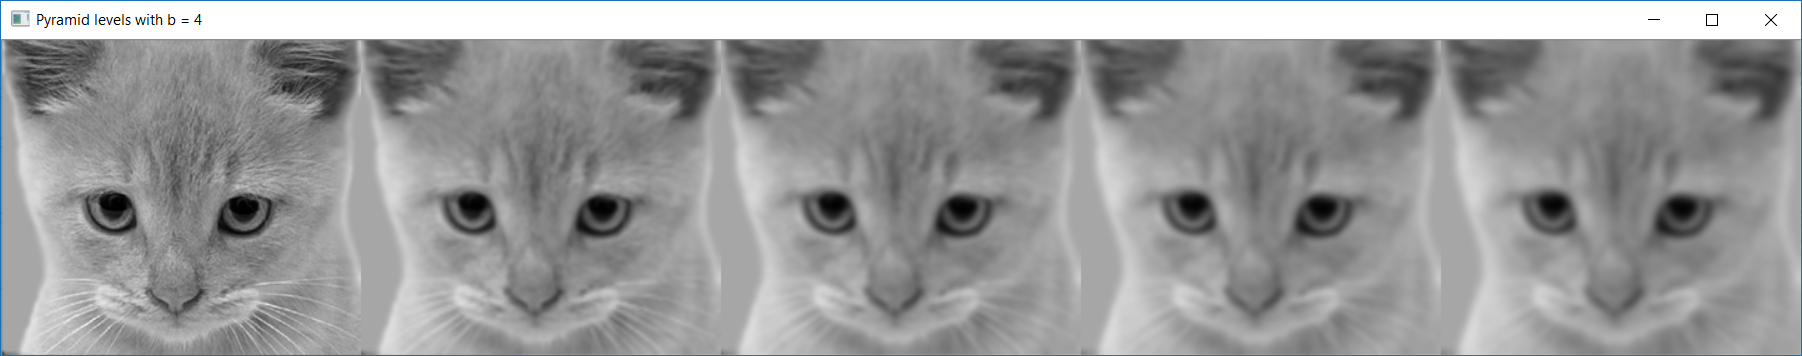
\includegraphics[scale=0.4]{2d1.PNG}
\caption{Pirámide Gaussiana de 4 niveles con bordes por defecto}
\end{figure}

\begin{figure}[h]
\centering
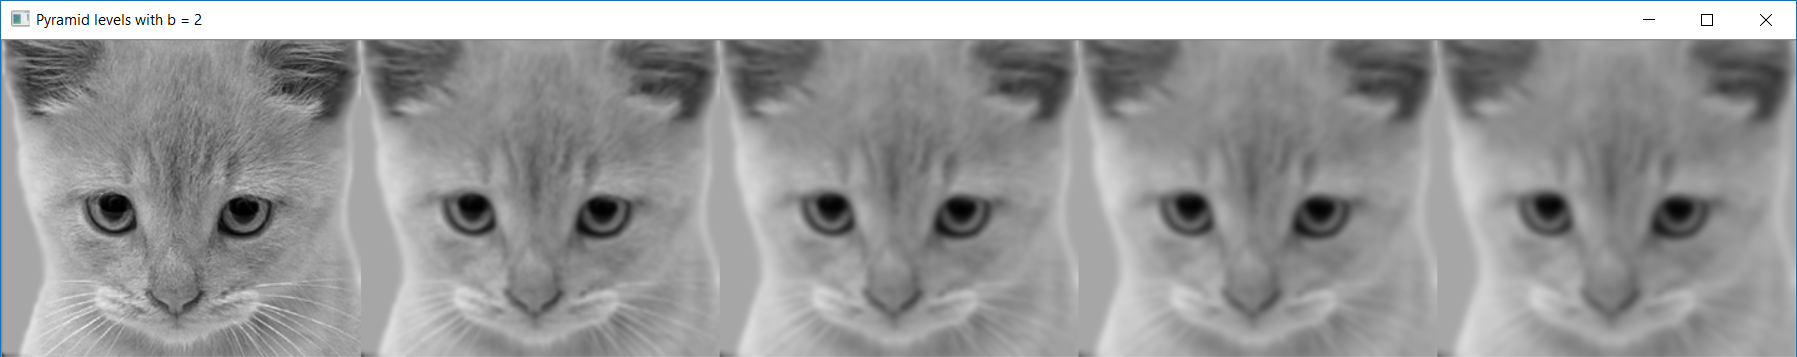
\includegraphics[scale=0.4]{2d2.PNG}
\caption{Pirámide Gaussiana de 4 niveles con bordes reflejados}
\end{figure}

\newpage
\subsection{Una función que genere una representación en pirámide Laplaciana de 4 niveles de una imagen. Mostrar ejemplos de funcionamiento usando bordes.}
En este caso hacemos una pirámide similar a la del ejercicio anterior en la que lo primero que debemos hacer es escalar la imagen original a una más pequeña y volverla a escalar al tamaño original. Una vez hecho esto tenemos la misma imagen que en el apartado anterior, una imagen con menos calidad y más difuminada. Con dicha imagen la restamos a la imagen original y de esta forma conseguimos eliminar las bajas frecuencias y hallar los bordes. Mientras iteramos sobre las imágenes modificadas vamos eliminando cada vez más información y al final encontramos una imagen con las fronteras más relevantes.

Para esta representación también se han usado dos bordes, el que nos ofrece por defecto OpenCV y el borde reflejado. Al igual que en el apartado anterior la diferencia apenas es apreciable.


\begin{figure}[h]
\centering
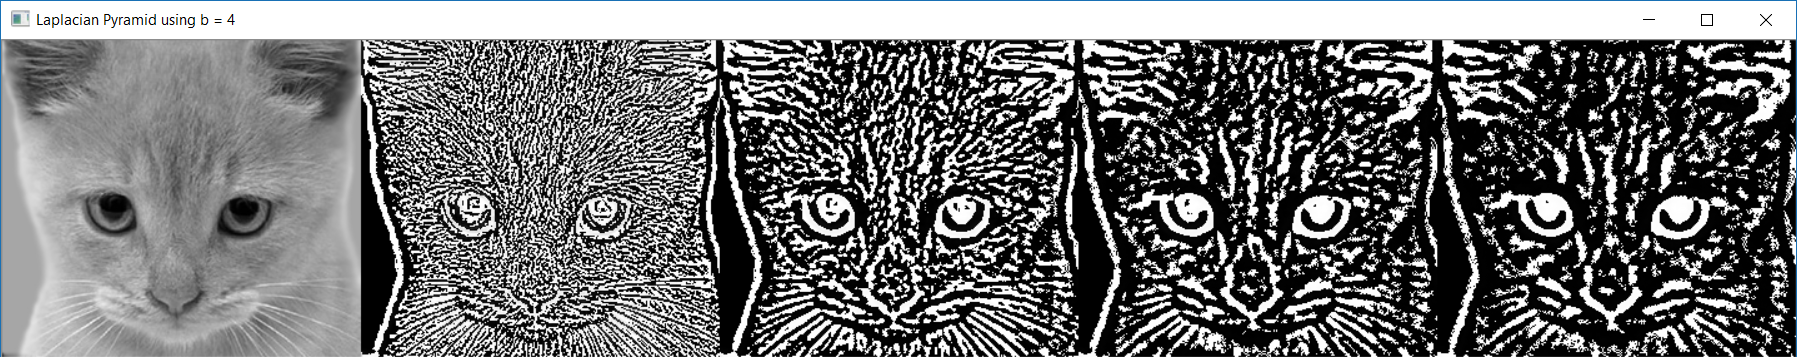
\includegraphics[scale=0.4]{2e1.PNG}
\caption{Pirámide Laplaciana de 4 niveles con bordes por defecto}
\end{figure}

\begin{figure}[h]
\centering
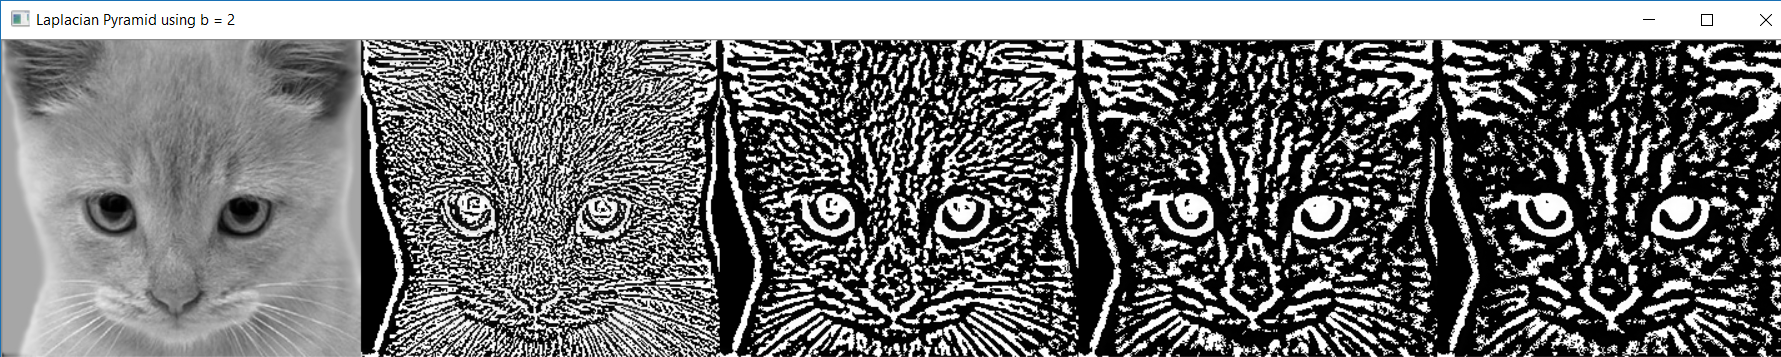
\includegraphics[scale=0.4]{2e2.PNG}
\caption{Pirámide Laplaciana de 4 niveles con bordes reflejados}
\end{figure}

\newpage
\section{Imágenes Híbridas}
Mezclando adecuadamente una parte de las frecuencias altas de una imagen con una parte de las frecuencias bajas de otra imagen, obtenemos una imagen híbrida que admite distintas interpretaciones a distintas distancias ( ver hybrid images project page). 

Para seleccionar la parte de frecuencias altas y bajas que nos quedamos de cada una de las imágenes usaremos el parámetro sigma del núcleo/máscara de alisamiento gaussiano que usaremos. A mayor valor de sigma mayor eliminación de altas frecuencias en la imagen convolucionada. Para una buena implementación elegir dicho valor de forma separada para cada una de las dos imágenes ( ver las recomendaciones dadas en el paper de Oliva et al.). 

Recordar que lasmáscaras 1D siempre deben tener de longitud un número impar. Implementar una función que genere las imágenes de baja y alta frecuencia a partir de las parejas de imágenes ( solo en la versión de imágenes de gris) . El valor de sigma más adecuado para cada pareja
habrá que encontrarlo por experimentación.


\subsection{Escribir una función que muestre las tres imágenes ( alta, baja e híbrida) en una misma ventana. (Recordar que las imágenes después de una convolución contienen número flotantes que pueden ser positivos y negativos)}


Para este apartado he optado por usar un filtro gaussiano con un tamaño de kernel variable que elegiremos en función del tamaño de las imágenes que queramos combinar para que el resultado se ajuste mejor. 
Con la misma máscara de alisamiento le aplicamos a una imagen el filtro para obtener las bajas frecuencias y con la otra imagen hacemos lo mismo para obtener las bajas frecuencias y restarselas a la original para obtener las altas. De esta forma ya tenemos nuestras dos imágenes con bajas y altas frecuencias, haciendo uso de la función \textit{add} de OpenCV las combinamos para obtener una imagen final que esté contenida en el rango (0, 1).



\newpage
\subsection{ Realizar la composición con al menos 3 de las parejas de imágenes}

Aquí podemos ver las distintas imágenes que se han obtenido usando la función del apartado anterior.

\begin{figure}[h]
\centering
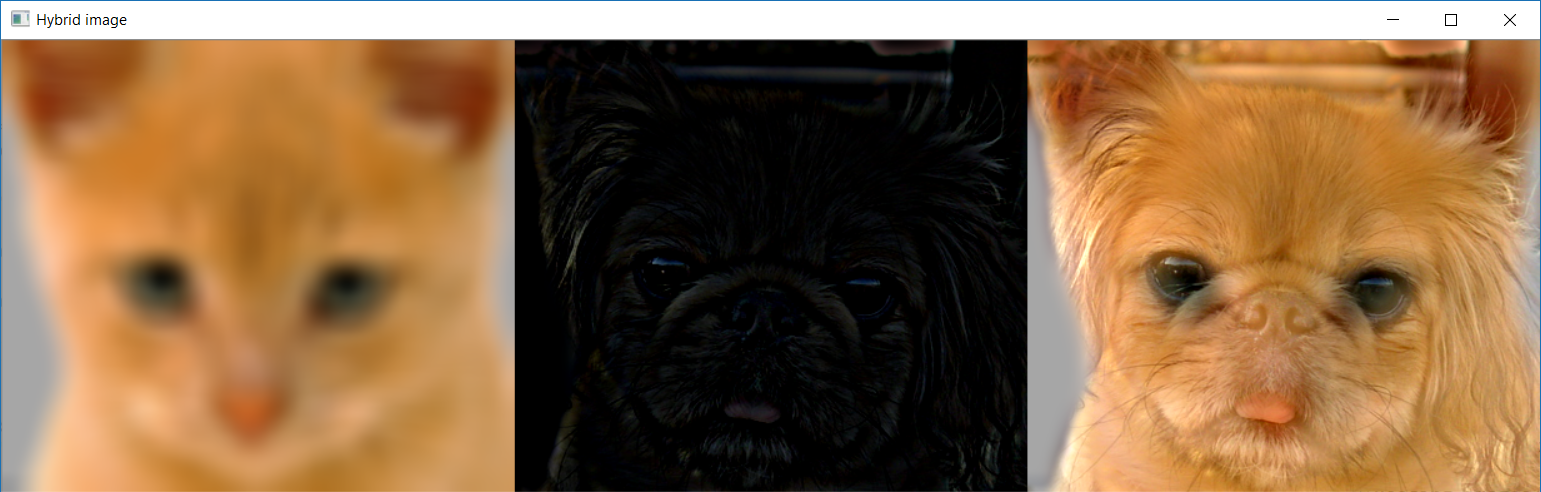
\includegraphics[scale=0.45]{3b1.PNG}
\caption{Gato y Perro}
\end{figure}

\begin{figure}[h]
\centering
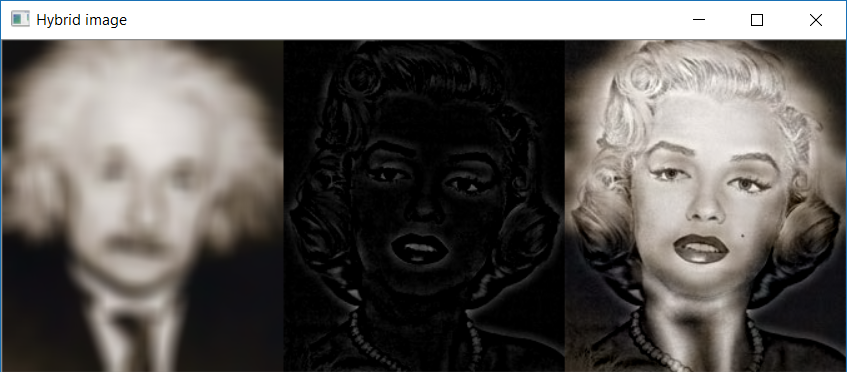
\includegraphics[scale=0.7]{3b2.PNG}
\caption{Einstein y Marilyn}
\end{figure}

\begin{figure}[h]
\centering
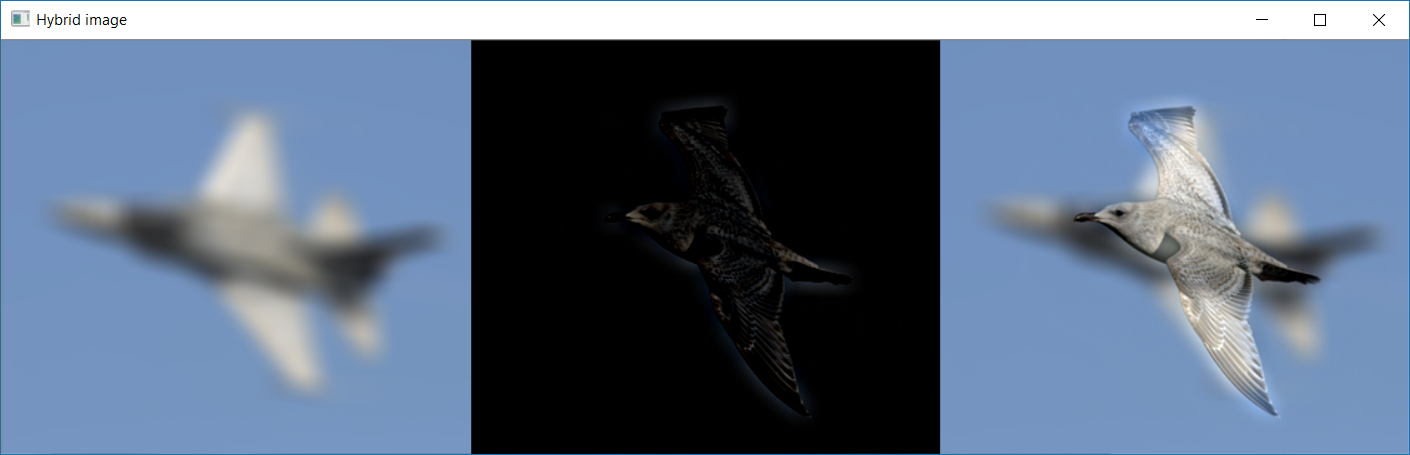
\includegraphics[scale=0.45]{3b3.PNG}
\caption{Avión y pájaro}
\end{figure}

\newpage
\begin{figure}[h]
\centering
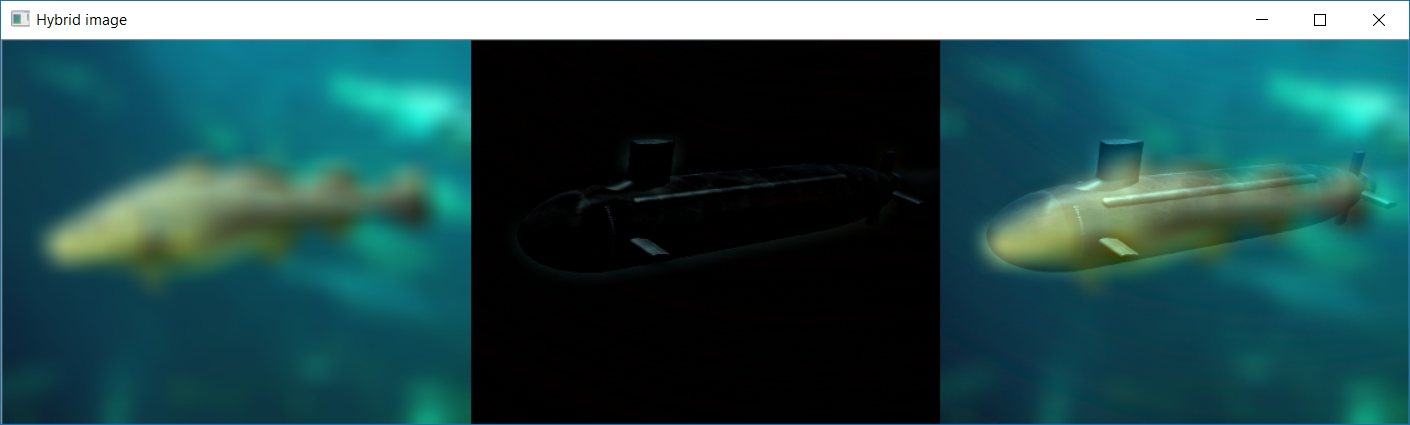
\includegraphics[scale=0.45]{3b4.PNG}
\caption{Pescado y submarino}
\end{figure}

\begin{figure}[h]
\centering
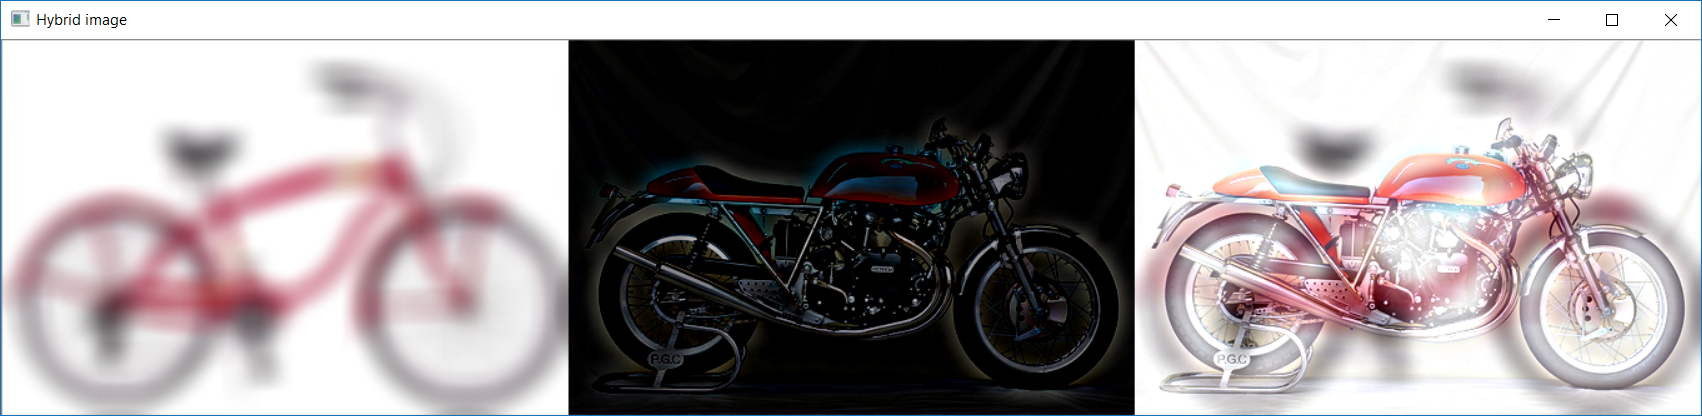
\includegraphics[scale=0.45]{3b5.PNG}
\caption{Bicicleta y Motocicleta}
\end{figure}



\end{document}
